\section{Related Work}
\label{sec:related}
When it comes to GNN interpretability, there are a few main methods. The first that started the field of GNN intepretability was GNN Explainer \cite{ying_gnnexplainer_2019} which also provided a suite of general benchmarks that most methods have utilized as a framework for analyzing the effecrtiveness of their explainer framework. Another major piece of work in the field has been the parametrized-graph explainer (PGExplainer) \cite{luo_parameterized_2020} that took GNNExplainer and parametrized it with a deep neural network for faster inference times and more robust interpretaiton. Along with these two, a few other more recent explainers such as SubgraphX \cite{yuan_explainability_2021} and Gem \cite{lin_generative_2021} have introduced new ideas into the field with a variety of approaches to the problem of GNN interpretability. To date, there seems to be no fully Bayesian method to the problem of GNN interpretability.

In addition to these works, the work of SERGIO \cite{dibaeinia_sergio_2020} will be introduced as it will be utilized later on to generate a new class of experiments that GNN Interpretability methods can be benchmarked against. This work provides causal graph structures that give a garunteed groundtruth for interpretation.

\subsection{GNN Explainer}
The full version of GNNExplainer attempts to learn both a node interpretation and edge interpretation. For this work, only the edge interpretation part of the framework was utilized. GNN Explainer attempts to solve the objective outlined in \S\ref{sec:intro-interp}, by only trying to learn $\mathcal{W}_i$ while treating $\mathcal{E}_i = E$. In this framework, GNN Explainer enforces that for any $e \in E$, $W(e) \geq \mathcal{W}_i(e)$. Then to get the argmax, GNNExplainer treats $\mathcal{W}_i$ as a random variable. Then the goal get transformed to 
\begin{align*}
	\argmin_{\mathcal{W}_i} \mathbb{E}_{w \sim \mathcal{W}_i} [H(\phi(v_i, \mathcal{X}, E, w))]
\end{align*}
This still remains intractible, so GNNExplainer attempts to make this simpler by using Jensen's inequality. Note that this is not a reasonable application of Jensen's since $\phi$ as a GNN has almost no hope of being convex. Nonetheless, using Jensen's inequality gives
\begin{align*}
	\argmin_{\mathcal{W}_i} H(\phi(v_i, \mathcal{X}, E, \mathbb{E}[\mathcal{W_i}]))
\end{align*}
This is still quite intractible if $\mathcal{W_i}$ is a full joint distribution over all $e \in E$. Therefore, GNNExplainer attempts to use a mean field approximation for $\mathcal{W}_i$ where the edge interpretation is decomposed into the product of Bernoulli distributions meaning that each edge weight is an independent Bernoulli distribution with mean equal to the underlying probabiltiy of the variable. Specifically,
\begin{align*}
	\mathcal{P}(\mathcal{W}_i) = \prod_{(v_j, v_k) \in E} \mathcal{W}_i[v_j, v_k]
\end{align*}
with each $\mathcal{W}_i[v_j, v_k]$ is a value between $[0, 1]$ representing a Bernoulli variable for each edge in the underlying graph as defined by $E$. In this case, if the classification for a node is $c$, GNNExplainer performs direct gradient descent on this array of values to minimize
\begin{align*}
	\argmin_{\mathcal{W}_i = \{\mathcal{W}_i[v_j, v_k] \mid (v_j, v_k) \in E\}} -\sum_{c=1}^C \mathbb{1}_{y = c} \log \mathcal{P}(\phi(v_i, \mathcal{X}, E, \mathcal{W}_i) = c)
\end{align*}
While there is some probabilistic formulation here, in effect, GNNExplainer optimizes an adjacency matrix in $[0, 1]$ against the mutual information of the model given the edge weights and the model with the original graph. This means that GNNExplainer learns no conditional structure between edges and does not take the graph dynamics into account while training. Hence, it is a pretty crude algorithm that provides only a summary of the interpretation using assumptions that are not generally applicable to GNNs.
\subsubsection{Benchmark Datasets}
As one of the first explainer methods for GNNs, GNNExplainer created a set of synthetic datasets that serve as the canonical datasets for GNN Interpretability. The goal of this section is to describe these datasets and the percieved shortcomings in these datasets that led to an exploration of their validity and a setup for the experiments produced later that demonstrate the incorrectness of these datasets for the stated task.

The main dataset focused on in this paper is the Tree-Cycles dataset \cite{ying_gnnexplainer_2019}. In this dataset trees of depth three are attached to cycles of length six in order to form and aggregate dataset. A GNN node classification task entails predicting whether a given node is either in a tree portion of the graph or in the cylcic portion of the graph with no given node features. The idea here is that the GNN can only rely upon the structure of the graph for its node classification and all its information must come from the edges. Hence interpretation on the edges of the GNN would reveal only information that could be gleaned from the graph structure. In figure \ref{fig:tree-cycles}, one can see an example of a portion of the dataset looking at a three-hop neighborhood around node 565.
\begin{figure}[t]
	\centering
	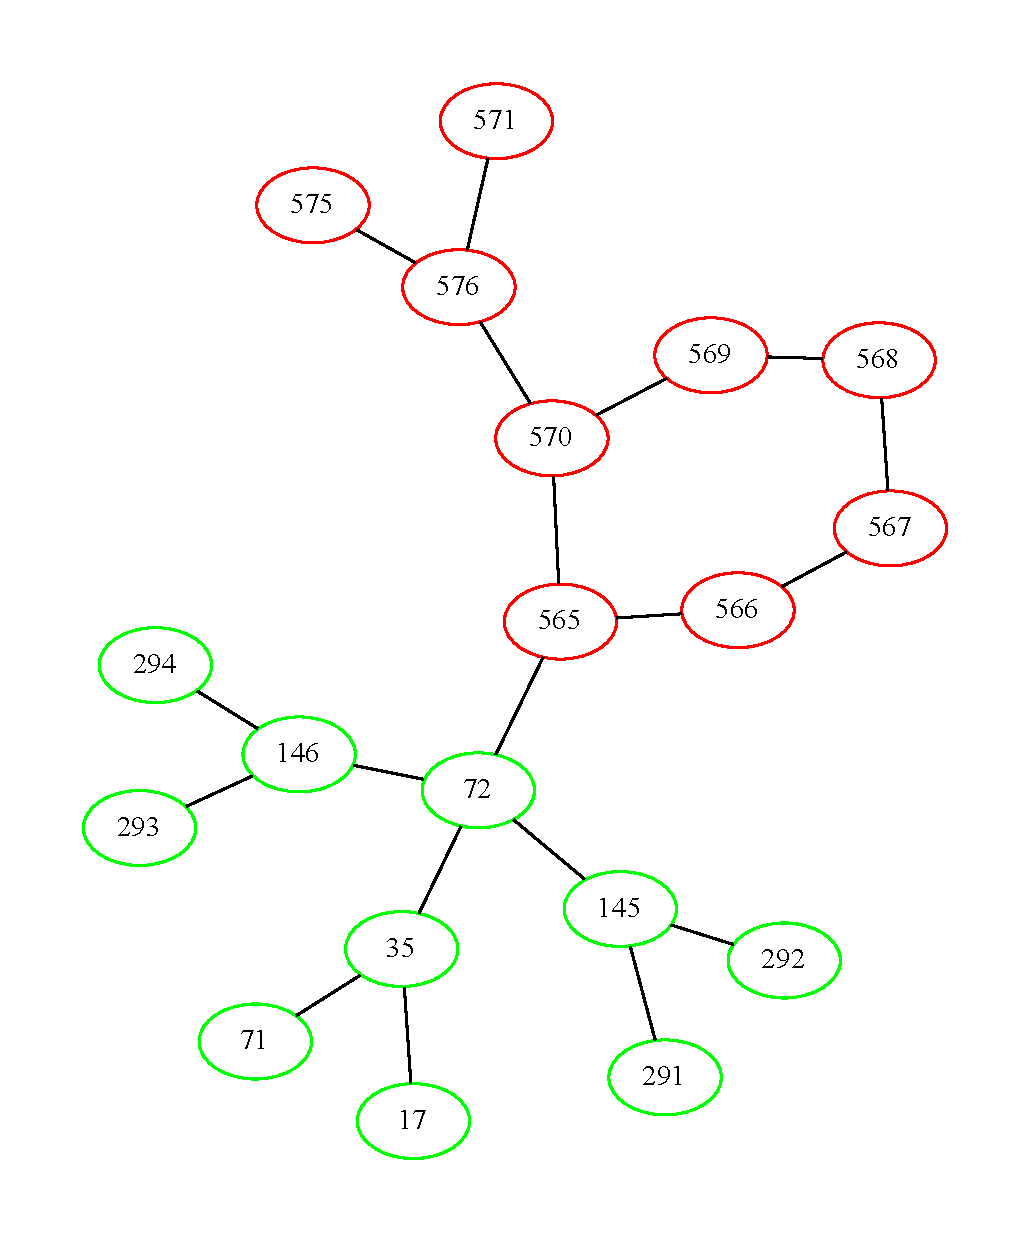
\includegraphics[width=0.6\textwidth]{images/tree-cycles.pdf}
	\caption{A look at the tree-cycles dataset at a three-hop neighborhood around node 565. In green are nodes classified as tree nodes and in red are nodes classified as cycle nodes. The dataset is almost 50\% balanced between these two types.}
	\label{fig:tree-cycles}
\end{figure}

\subsection{Parametrized-Graph Explainer}

\subsection{Other Explainer Frameworks}

\subsection{SERGIO}

